\chapter{Uncertainty and Risk Management}
\label{chap:risk}
We translate predictive uncertainty into portfolio-level risk controls, ensuring that betting strategies remain resilient under changing market conditions.\mndown{2}{Quantify, propagate, and govern model uncertainty; see Kelly staking~\S\ref{sec:kelly-math}, CVaR program~\S\ref{sec:cvar-math}, and lattice CRPS~\S\ref{subsec:crps-lattice}.}

% --- Mathematical reasoning: uncertainty and risk ---
\section{Kelly criterion and fractional scaling}\label{sec:kelly-math}
Following \citet{kelly1956}, for edge $p$ at decimal odds $b+1$, the log-growth maximizing fraction is $f^\star=p-(1-p)/b$; fractional Kelly $\kappa f^\star$ trades growth for risk.
For a binary bet with net decimal odds $b>0$ and true win probability $p$, staking fraction $f$
maximizes expected log growth:
\begin{equation}\label{eq:kelly-opt}
f^\star=\argmax_{f\in[0,1]}\; p\log(1+fb)+(1-p)\log(1-f)
= p - \frac{1-p}{b}.
\end{equation}
Fractional Kelly $\tilde f=\kappa f^\star$ with $\kappa\in(0,1]$ trades growth for lower variance
and smaller drawdowns; we report sensitivity over $\kappa$.

\subsection{Parameter uncertainty: posterior–lower–bound Kelly}\label{subsec:bayes-kelly}
With estimated probabilities, maximizing Bayesian expected log growth reduces to plugging the posterior mean $\bar p=\E[p\mid\mathcal D]$ into \eqref{eq:kelly-opt}. To account for estimation risk conservatively, we stake on a \emph{lower credible bound} for $p$:
\begin{align}\label{eq:lcb-kelly}
&p_{\text{LCB}}=\text{Quantile}_{\alpha}\big(p\mid \mathcal D\big)\quad\text{(exact Beta or normal approx. }\bar p - z_{\alpha}\,\sqrt{\Var[p\mid\mathcal D]}\text{)},\\
&f_{\text{LCB}}=\left[\,\frac{(b+1)\,p_{\text{LCB}}-1}{b}\,\right]\_{[0,1]},\qquad b=\text{decimal odds}-1,
\end{align}
and optionally apply fractional scaling $\tilde f=\kappa f_{\text{LCB}}$. We use $\alpha\in[0.05,0.10]$ and report sensitivity. This makes the role of posterior variance explicit and guards against overbetting when uncertainty is high.

\subsection{Kelly with friction and caps}\label{subsec:kelly-friction}
If the effective net odds are $b' = b - \tau$ due to fees/slippage/taxes and stake is capped at $c$,
the optimal unconstrained $f^\star=p-(1-p)/b'$ is projected to $[0,c]$. Set $f=0$ if $b'\le 0$.
We report the sensitivity of growth to $\tau$ and $c$.

\begin{example}[Worked friction example]
If the posted decimal odds are 1.91 (typical -110), the net $b=0.91$. With true win probability $p=0.55$ and slippage $\tau=0.03$, the effective net is $b'=0.88$. The unconstrained Kelly is $f^\star=0.55-(0.45/0.88)\approx 0.039$. With a cap $c=0.02$, we stake $f=0.02$ (2\% of bankroll).
\end{example}

\subsection{Approximate ruin probability}\label{subsec:ruin}
Under small stakes per bet, $\log W_t$ behaves like a random walk with drift $\mu_G$ and variance
$\sigma_G^2$ per bet. With lower barrier $L=\log W_{\min}$, the probability of ever hitting $L$ is
approximately $\exp\!\big(-2(\log W_0-L)\mu_G/\sigma_G^2\big)$ when $\mu_G>0$.

\section{CVaR-constrained stake sizing}\label{sec:cvar-math}
Let $L$ be portfolio loss over a horizon. At level $\alpha$, $\mathrm{CVaR}_\alpha=\E[L\mid L\ge \mathrm{VaR}_\alpha]$.
Given predictive draws $\{R^{(b)}\}_{b=1}^B$ for per-bet returns and stake vector $\vect f$, the convex
program
\begin{align}
\min_{\vect f,\,t,\,\xi_b\ge0}\quad & t+\frac{1}{(1-\alpha)B}\sum_{b=1}^B \xi_b \label{eq:cvar-prog}\\
\text{s.t.}\quad & \xi_b \ge -\vect f^\top R^{(b)} - t,\; b=1,\dots,B,\qquad \vect f\in\mathcal{F} \nonumber
\end{align}
limits tail risk while allowing Kelly-like growth on the interior. We include exposure/market caps in $\mathcal{F}$.

\begin{theorem}[Convexity of Rockafellar--Uryasev CVaR program \citep{rockafellar2000}]
The optimization problem \eqref{eq:cvar-prog} is convex in $(\vect f, t, \xi)$ since the objective is linear and constraints are affine, ensuring global optimality and tractability.
\end{theorem}

\textit{Proof sketch:} The objective is a sum of linear terms, and the constraints define a convex feasible set via affine inequalities. Thus, the program is a convex optimization problem.

\subsection{Computational complexity and wall-clock}
Let $n$ be the number of positions and $B$ the number of Monte Carlo scenarios. Program~\eqref{eq:cvar-prog} is a linear program with $n+1+B$ variables and $B$ scenario constraints plus any position constraints in $\mathcal{F}$. Worst-case bounds for generic interior-point methods are polynomial (e.g., $\tilde O((n+B)^3)$ arithmetic operations), but they are loose here. The constraint matrix is extremely sparse (one nonzero per position in each scenario row), and practical solvers exploit this: per-iteration cost is \emph{linear in $B$} with small constants.

Implementation details and benchmarks. We solve \eqref{eq:cvar-prog} with CVXPy backends (HiGHS/ECOS/MOSEK) and warm-start across folds and weeks. On a laptop-class CPU, representative instances with $n\in[50,200]$ and $B\in[5\times10^3,5\times10^4]$ complete in sub-second wall-clock; warm-starts reduce repeat solves to tens–hundreds of milliseconds. Scaling is near-linear in $B$ until memory bandwidth dominates. Batching scenarios or using stochastic subgradient approximations caps latency for very large $B$.

\section{Uncertainty Quantification}
\begin{itemize}
  \item \textbf{Bayesian posteriors:} analytic draws from linear-Gaussian models provide closed-form intervals.
  \item \textbf{Bootstrap ensembles:} resampling-based variance estimates capture feature and model instability for ML components.
  \item \textbf{Simulation diagnostics:} posterior predictive checks highlight distributional misspecification.
\end{itemize}

\section{Portfolio Perspective}
We frame multiple concurrent bets as a portfolio with covariance driven by shared model features and market conditions. We approximate correlation using historical co-movements of CBV and implied probabilities, and bound exposure so that total variance remains below the weekly risk budget.

\section{Stake Sizing Policies}
Fractional Kelly staking is adjusted via credible intervals to produce cautious positions when uncertainty inflates. We also explore utility-based objectives (power utility, log utility with drawdown penalty) to tailor aggressiveness to stakeholder preferences.

\subsection{Kelly and Fractional Kelly}
For an edge \(e\) at odds \(o\), Kelly fraction \(f^* = \frac{(o-1)p - (1-p)}{o-1}\) maximizes expected log wealth. We adopt fractional \(\lambda f^*\) with \(\lambda \in (0,1)\) calibrated to uncertainty: \(\lambda\) is reduced when posterior variance widens or portfolio concentration increases.

\subsection{Drawdown Analytics}
We estimate expected maximum drawdown under the posterior predictive distribution using block bootstrap of weekly returns. Policies are accepted only if drawdown quantiles remain within governance thresholds. This conservative screen meaningfully lowers tail risk at the cost of modestly slower growth.

\begin{figure}[t]
  \centering
  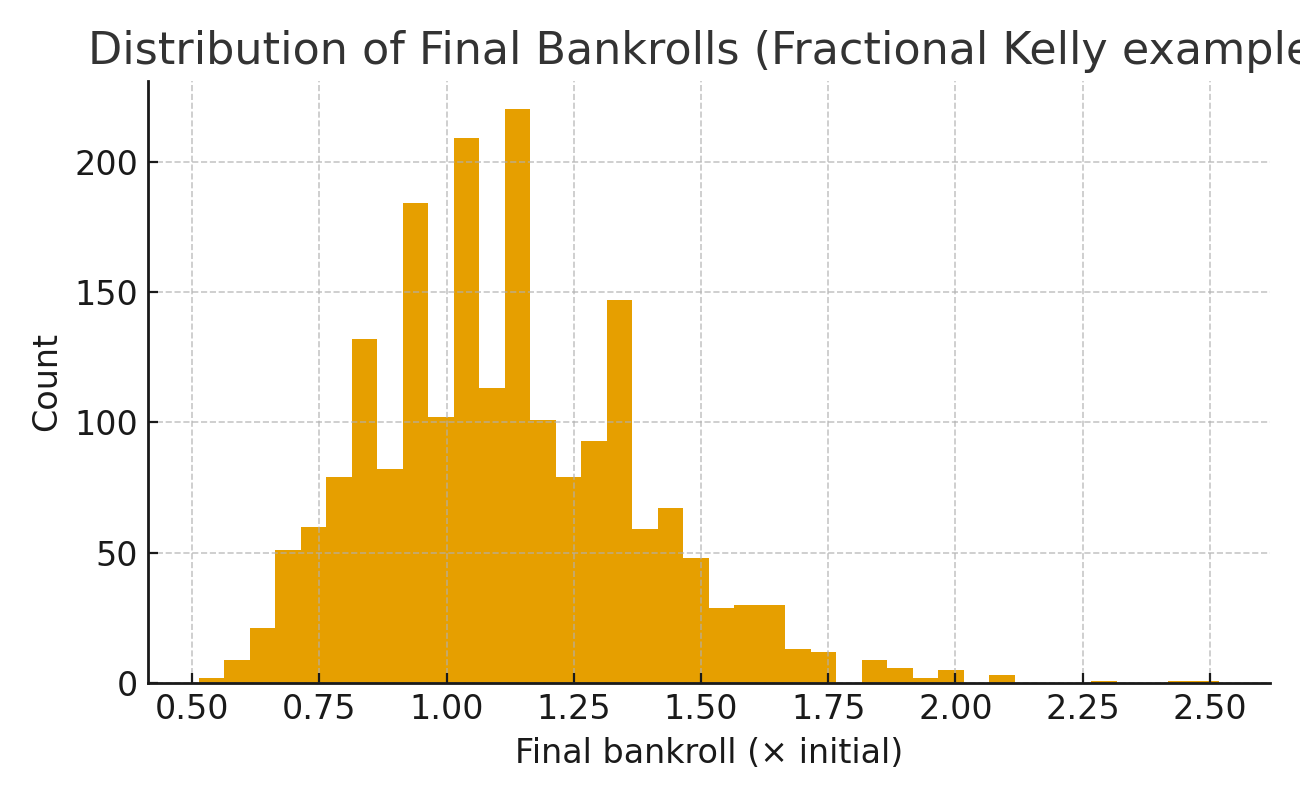
\includegraphics[width=0.9\linewidth]{../figures/bankroll_hist.png}
  \caption{Distribution of final bankroll outcomes under the drawdown-screened policy. Each bar aggregates Monte Carlo runs after applying fractional Kelly caps and CVaR gating.}
  \label{fig:bankroll-hist}
\end{figure}

\section{Governance and Reporting}
A risk committee reviews weekly dashboards summarizing realized vs expected variance, tail losses, and limit breaches. Automated alerts trigger when realized drawdown surpasses modeled expectations, pausing RL policy execution until manual review.

\chaptersummary{
We connected predictive uncertainty to decision‑making via fractional Kelly with friction/caps, CVaR‑constrained stake sizing, and portfolio‑aware exposure limits. Diagnostics and governance (variance tracking, drawdown alerts) anchor safe deployment and directly support the thesis that uncertainty + governance convert edge into reliable growth.
}{
Chapter~\ref{chap:sim} uses these risk‑aware policies in a Monte Carlo simulator that prices teasers/middles, models frictions and dependence, and evaluates robustness before risking capital.
}

\todo{Include example dashboard snapshot of variance decomposition.}

\section{Correlation Estimation}
We estimate pairwise correlations from historical co‑movements in CBV and implied probabilities and regularize using shrinkage toward sparse structures. Sensitivity to correlation misspecification is evaluated by worst‑case bounds that inform exposure caps.

\section{Kelly Examples}
We include worked examples with varying edge, odds, and variance to illustrate fractional Kelly and the impact of uncertainty gating on stake sizes. When variance doubles, stake fractions are halved or more depending on tail sensitivity.

\begin{figure}[t]
  \centering
  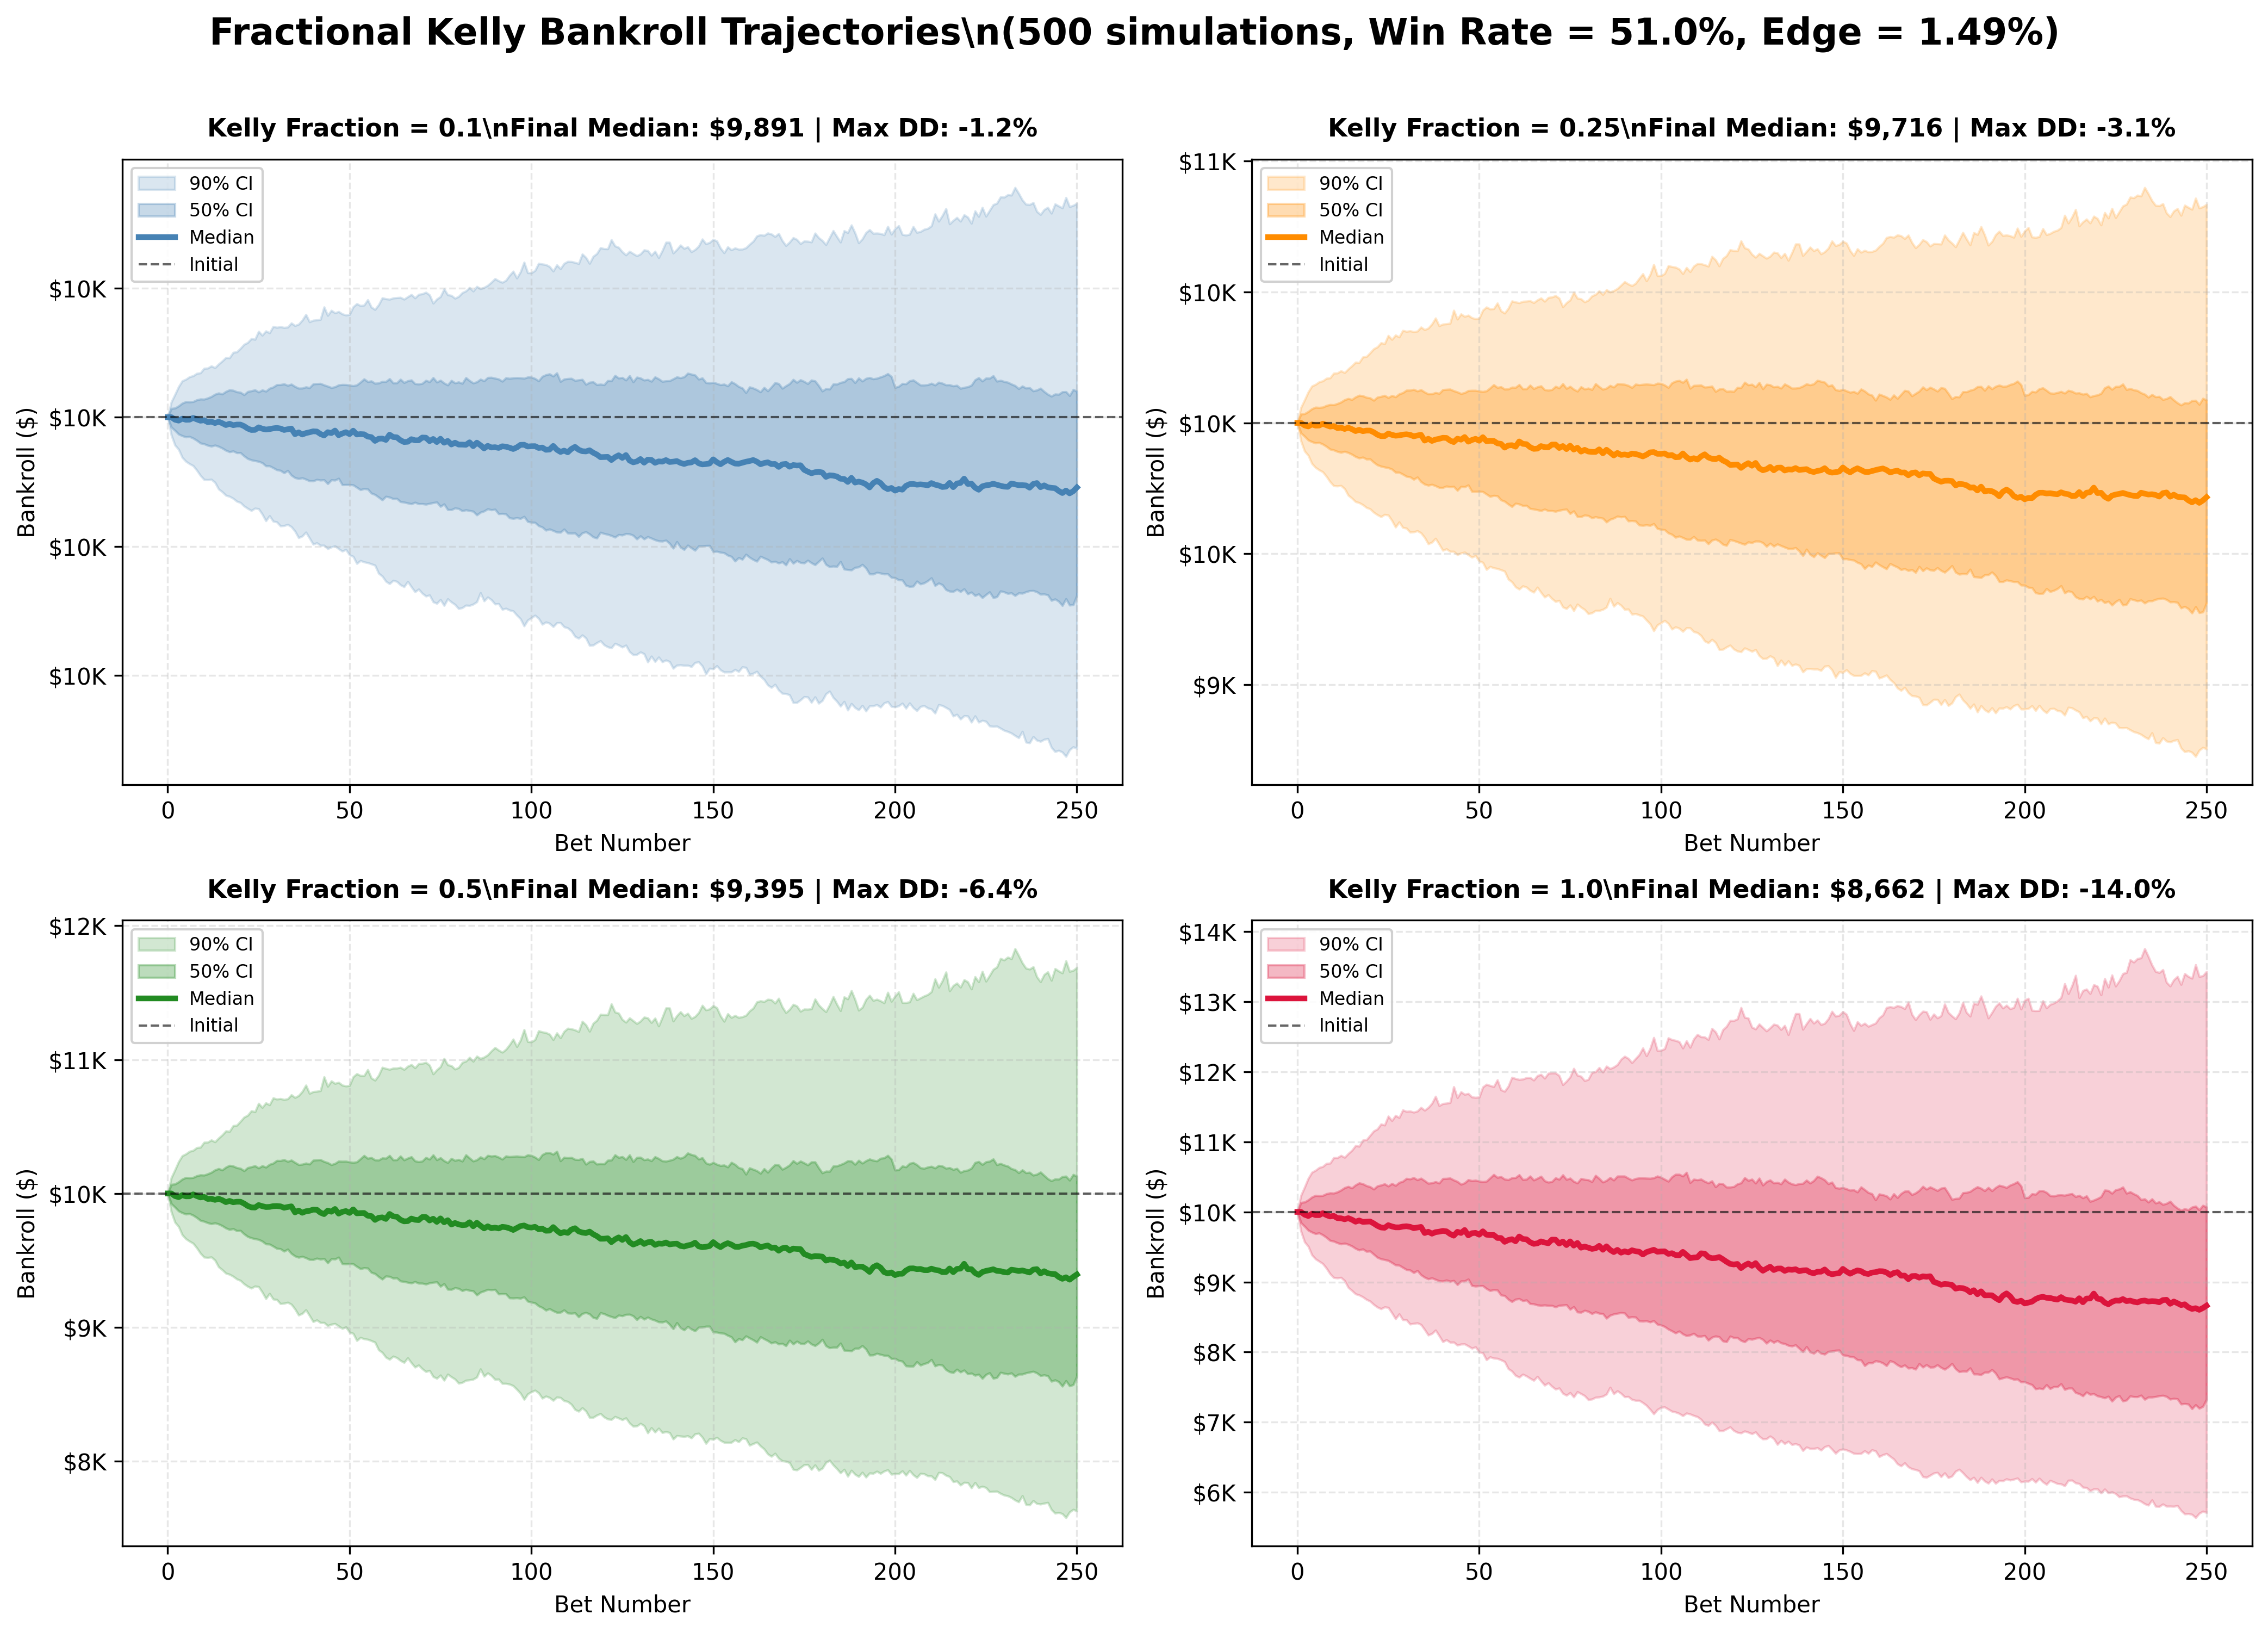
\includegraphics[width=0.9\linewidth]{../figures/bankroll_trajectories.png}
  \caption{Simulated bankroll trajectories under fractional Kelly multipliers. Lines show median paths with 50\% and 90\% credible envelopes, highlighting the growth versus drawdown trade-off.}
  \label{fig:bankroll-trajectories}
\end{figure}

\section{CVaR Implementation}
We compute CVaR via posterior predictive draws on weekly returns. Policies are accepted if CVaR at the chosen confidence remains within budget. Optimization solves a convex approximation with variance and CVaR constraints.

% Example margin note placement near CVaR equations
% (removed former margin-note guidance)
\begin{algorithm}[t]
  \caption{CVaR Stake Sizing with Warm Starts}
  \label{alg:cvar-solve}
  \begin{algorithmic}[1]
    \Require scenario returns $R^{(b)}\in\mathbb{R}^n$ ($b=1..B$); confidence $\alpha$; feasible set $\mathcal F$; previous solution $(\vect f_{\text{prev}},t_{\text{prev}})$ (optional)
    \Ensure stakes $\vect f\in\mathcal F$, CVaR estimate
    \State Build LP in variables $(\vect f,t,\{\xi_b\})$ with constraints $\xi_b\ge-\vect f^\top R^{(b)}-t$ and $\vect f\in\mathcal F$
    \State Warm‑start with $(\vect f_{\text{prev}},t_{\text{prev}})$ if available; otherwise use capped Kelly baseline
    \State Solve LP with interior‑point or simplex; cache factorization for nearby problems
    \State Return $\vect f$ and CVaR $t+\frac{1}{(1-\alpha)B}\sum_b \xi_b$
  \end{algorithmic}
\end{algorithm}
